\chapter{Running the PR2}
Running the PR2 requires a basic understanding of ROS (\href{http://www.ros.org}{http://www.ros.org}), the BSD-licensed 
Robot Operating System.  A ROS system consists of multiple processes running on multiple computers.  If you are not 
familiar with ROS, it is highly recommended that you follow some of the \href{http://www.ros.org/wiki/ROS/Tutorials}{beginner tutorials} 
on ros.org. Familiarity with ROS tools will make using the robot much easier.  In particular, you should understand 
what a launch file is and how to run it, and how to run ROS with nodes on multiple computers. This chapter will walk 
you through starting up and running a PR2, using ROS.

\section{Getting set up}
\subsection{Out of the box}
If you are starting your PR2 for the first time at your institution, please read the previous chapter, \ref{Setting up PR2 in your lab}.  
This will give you advice on setting up the network, setting the administrative password, and picking a safe location for 
charging the PR2.  This chapter assumes that the PR2 is already set up for your lab.
\subsection{Batteries and power}
Before running the robot, you need to make sure it has power, which is easiest to do by making sure the robot is plugged in to a wall outlet. You can follow the instructions in this chapter to start up the PR2 while it is plugged into the power outlet, which will keep the batteries charged.  The battery life of the PR2 is approximately two hours, so it is a good idea to keep the PR2 plugged in when not in use.  

%Add instructions about Ethernet being plugged in, too? User#2 recommended to add this information.

\subsection{Run-stop}
Before running the robot, you should also have the wireless run-stop 
nearby (Figure~\ref{fig:runstop}), so that you can shut down the motors if you need to. 

The PR2 has two run-stop buttons: the red push-button on the middle of the PR2's back, and 
the yellow wireless run-stop transmitter. If either one is in the stop position, the motors are disabled so the
robot cannot move. {\bf In an emergency, press the stop button on the wireless transmitter, or
hit the push-button in the back}. Putting either run-stop button in the stop position does not
damage the robot or turn off the computers, it simply stops the motors.


%Add image of red push-button on PR2's back here
\begin{figure}[h]
\centering
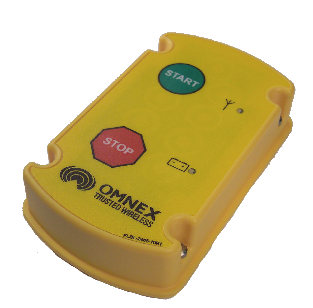
\includegraphics[width=150px]{run_stop.png}
\caption{The PR2 wireless run-stop.}
\label{fig:runstop}
\end{figure}

The wireless run-stop is also powered by batteries, which can run down.
Therefore, it is a good idea anyway to turn the wireless run-stop off (by pressing the "STOP" button) when not in use.
If the wireless run-stop runs out of battery charge, then the battery light
(the light next to the battery symbol in the lower half of the wireless run-stop face)
will flash. To change the battery, you will need a slotted screwdriver to open
the wireless run-stop case (Figure~\ref{fig:opening-runstop}).

\begin{figure}[!h]
\centering
\includegraphics[width=125px]{opening_runstop.png}
\caption{Opening the PR2 wireless run-stop to change the batteries.}
\label{fig:opening-runstop}
\end{figure}

\subsection{Getting an account}
Before using the PR2, you will also need an account on the robot computers. Ask the robot administrator to create an account for you, using the instructions 
in section \ref{creating accounts}.
\section{Turning on PR2}
If the robot is already running, you can skip this step, but you should still put the wireless run-stop in the stop position. 

To turn the PR2 on, you should first verify that the wireless run-stop is in the stop position. If it is not yet in the stop position, then press the wireless run-stop's red ``STOP'' button; the lights on the wireless run-stop should turn off. 

Second, switch the red run-stop button on the back panel of the robot to the ``on'' position; turn it clockwise and it will pop out.

Third, if the DC breaker switch at the back panel of the robot is switched off, then flip the DC breaker switch (Figure~\ref{fig:dc_breaker}) to the ``on'' position.

\begin{figure}[h]
\centering
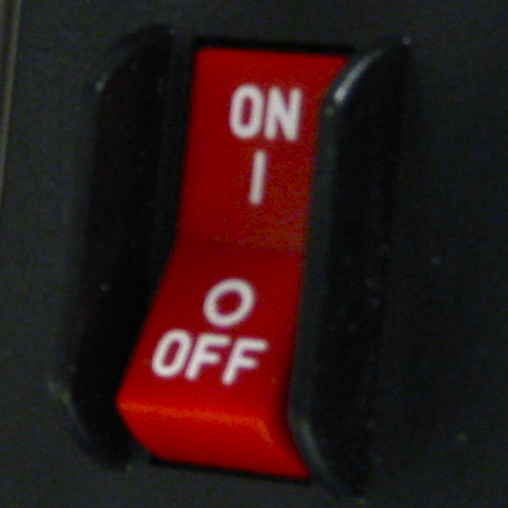
\includegraphics[width=50px]{dc_breaker.png}
\caption{The PR2 DC breaker switch in the ON position.}
\label{fig:dc_breaker}
\end{figure}

You should see the red lights on the computers turn on, hear the fans spin up, and hear several rising-tone beeps from the computers 
as they boot.  The process of booting the computers will take about 5 minutes.  You will know that the computers are on when you see a red light illuminate on each of the computers in the robot base.  
\subsection{Logging in}
Once the robot is on, \texttt{\href{http://unixhelp.ed.ac.uk/CGI/man-cgi?ssh}{ssh}} into the main computer using the account 
created for you by the administrator, using the steps below.

In the following tutorial, we will use pr\textless x\textgreater 1 to refer to the first computer on robot \textless x\textgreater\ and \textless username\textgreater\ to refer to your account username.
Ask your robot  administrator what name you should use for the robot you want to run. 

To log in to the robot, open a terminal window and type
\begin{verbatim}
$ ssh <username>@pr<x>1
\end{verbatim}
You should already have access to all the ROS tools. For instance, to see what packages are available to you, type
\begin{verbatim}
$ rospack list-names
\end{verbatim}
and you should see a list of the ros packages currently in your path.

\subsection{Checking for other users}
If you logged in to a robot that was already running, you should check to see if anyone else is using the robot. To 
find out who else is using the robot, type
\begin{verbatim}
$ ckill list
\end{verbatim}
This will show you what programs are currently running on the robot.  If nothing shows up, then no one else is logged into the robot. If other people have processes running on the 
robot, you will need to find out if you can interrupt their work. You should find out who is on the robot and ask them 
to allow you to kill their processes so that you can work on the robot.  If you cannot find the people running processes 
on the robot, ask the robot adminstrator for guidance on what the policy is in your lab. If it is fine for you to kill 
the other processes running on the robot, you can type
\begin{verbatim}
$ sudo robot stop
\end{verbatim}
and all the processes that are being run on the robot will be killed.

\section{Starting the software}
The launch file /etc/ros/robot.launch is used to start up the basic functionality of the robot.  This includes drivers for 
the sensors, motors, speakers, projector, power system, and joystick as well as the default set of realtime controllers, 
processing and logging of diagnostics information, and monitors for various types of problems your robot could experience.  On a new robot, this launch file is standard, but if the robot you are working on has been altered (e.g., has additional sensors, has only one arm), then it is likely that someone administering the robot has also updated the /etc/ros/robot.launch file to work with your robot's configuration.

There are two ways to start the software on the PR2. The first way is easier than the second way.
 \subsection{Starting the software the easier way}

Once you are logged in and ready to start the robot, you can run the robot by typing
\begin{verbatim}
$ sudo robot start
\end{verbatim}
Running robot start will start the roslaunch for you in the background as a system user. This will 
allow you to continue to use your current terminal and the robot will keep running after you log out.  

To see what topics are being published in ROS now, you can type 
\begin{verbatim}
$ rostopic list
\end{verbatim}
This is a good way to check to see if you started up ROS successfully.

\subsection{Starting the software the manual way}
As an alternative to starting the software the easier way, you can also start the software manually. If you prefer to see everything that is going on, you can also start the robot software manually, but you will need to keep that 
window open until you are done using the robot. Closing that the terminal in which you roslaunched will terminate the roslaunch.
\begin{verbatim}
$ roslaunch /etc/ros/robot.launch
\end{verbatim}
to start up the pr2.  

If you used ``roslaunch'' to start the robot, then you will need to open a new terminal and type
\begin{verbatim}
$ ssh <username>@pr<x>1
$ rostopic list
\end{verbatim}
to see what topics are being published by the system in the new terminal while the roslaunch continues to run in the 
original terminal. Remember that \textless x\textgreater\ is a placeholding variable to be replaced with the ID of the robot you are using.

Either way, the robot should be running, but since you have the wireless run-stop in the stop position, the motors will not be moving.  

\section{Running the dashboard}
When running the robot, the pr2\_dashboard should always be up on your screen.  This is how the robot software will 
let you know if something is going wrong, and is also how you turn the motors and power on and off.  

On a computer with a built ROS installation (e.g., the base-station desktop computer that ships with the robot), not on the robot itself, set your ROS\_MASTER\_URI to point at the master running on the robot and launch the dashboard by typing
\begin{verbatim}
$ export ROS_MASTER_URI=http://pr<x>1:11311
$ rosrun pr2_dashboard pr2_dashboard
\end{verbatim}
You should see the pr2\_dashboard control panel (a graphical user interface) appear and provide you with information about the state of the robot. It is ok if not all of the icons are green. In fact, the run-stops should be ``warning'' you that the wireless runstop is not on.\footnote{If you do not see the pr2\_dashboard control panel appear, then there is a chance that you have not yet built the pr2\_dashboard. 
To do this, type \texttt{rosmake pr2\_dashboard} to build pr2\_dashboard. Once this is done, you can try launching the dashboard again.}

Take a moment to review the state of the robot. You can get a sense for the health of 
your robot by looking at the diagnostics information; click on the wrench on the far left.  Since you have the run-stop in the
stop position, you see that the motors are giving you a warning because the robot was just turned on and the encoders on the joints have not 
been calibrated yet. 
% (CURRENTLY THIS IS AN ERROR.  SHOULD CHANGE TO WARNING BY ROBOT SHIP DATE)

If you see warnings or errors in any other sections, you should read the error messages and try to figure out what the 
problem is.  Ask your robot administrator for help if there are errors that you do not understand.
\subsection{Understanding pr2\_dashboard}
When running the PR2, the most important piece of software for you to understand and control the state of the system is 
the pr2\_dashboard. pr2\_dashboard, Figure~\ref{fig:dashboard1}, is a GUI for debugging and controlling low-level state 
of the PR2. The dashboard displays the diagnostic, circuit breaker, run-stop, and battery status.
%\begin{figure}[h]
%\centering
%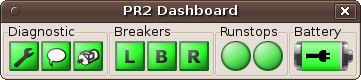
\includegraphics[scale=0.5]{pr2_dashboard.png}
%\caption{The PR2 dashboard when all is well.}
%\label{fig:dashboard}
%\end{figure}
\begin{figure}[h]
\centering
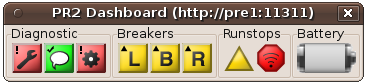
\includegraphics[scale=0.5]{dashboard1.png}
\caption{The PR2 dashboard when starting up the robot.}
\label{fig:dashboard1}
\end{figure}
The robot will not usually start up with all green lights. In fact, if you bring up the robot properly, then you should see a dashboard display that looks more like Figure~\ref{fig:dashboard1}.
This is because the wireless run-stop should be in the stop position.
You can tell that the wireless run-stop is in the stop position by mousing over the dashboard to see the tooltips, which describe what each icon means. See Figure~\ref{fig:dashboard2}.

\begin{figure}[h]
\centering
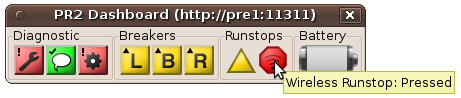
\includegraphics[scale=0.5]{dashboard2.png}
\caption{The PR2 dashboard when starting up the robot, showing tooltips.}
\label{fig:dashboard2}
\end{figure}

The following sections describe the other information displayed in the
dashboard.  Some of the indicators in the dashboard can have a status
of ``stale.''  This means that some component of the robot has stopped
reporting status information.  A stale status is usually caused by a
network problem (e.g., bad wireless connection from the base station to the
robot).


\begin{description}
\item[Diagnostic Status] The state of the robot is shown by the diagnostic indicators in the pr2\_dashboard. \\

    \newcolumntype{S}{>{\centering\arraybackslash} m{.9cm} }%
    \begin{tabular}{m{6cm}SSSS}
    Component & OK & Warn & Error & Stale\\
    &&&&\\
    Diagnostics: Clicking pops up the Robot Monitor & 
\includegraphics[scale=0.5]{diag_ok.png}&
\includegraphics[scale=0.5]{diag_warn.png}&
                                                      
\includegraphics[scale=0.5]{diag_error.png}&
\includegraphics[scale=0.5]{diag_stale.png}\\
    &&&&\\
    Rosout: Clicking pops up rxconsole & 
\includegraphics[scale=0.5]{rosout_ok.png}&
\includegraphics[scale=0.5]{rosout_warn.png}&
                                        
\includegraphics[scale=0.5]{rosout_error.png}&
\includegraphics[scale=0.5]{rosout_stale.png}\\
    &&&&\\
    Motors: Clicking allows you to halt or reset motors & 
\includegraphics[scale=0.5]{motor_ok.png}& N/A &
                                                          
\includegraphics[scale=0.5]{motor_error.png}&
\includegraphics[scale=0.5]{motor_stale.png}\\
   \end{tabular}

\item[Circuit Breaker Status] The circuit breakers are labeled L/B/R, which stand for Left Arm, Base/Spine, and Right Arm. 
Each breaker can be in one of four states, and clicking on any of the breakers will pop up a menu (Figure~\ref{fig:breaker_menu}), allowing you to change the state of one or all of them:
\begin{figure}[h]
\centering
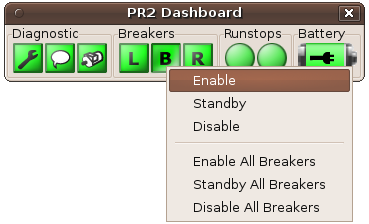
\includegraphics[scale=0.5]{breakers_menu.png}
\caption{The circuit breaker options menu.}
\label{fig:breaker_menu}
\end{figure}

    \newcolumntype{S}{>{\centering\arraybackslash} m{1.7cm} }%       
    \begin{tabular}{m{2.6cm}SSSS}
     & Enabled & Standby & Disabled & Stale\\
    Breaker Status & 
\includegraphics[scale=0.5]{L_ok.png}
\includegraphics[scale=0.5]{B_ok.png}
\includegraphics[scale=0.5]{R_ok.png}&
                     
\includegraphics[scale=0.5]{L_stby.png}
\includegraphics[scale=0.5]{B_stby.png}
\includegraphics[scale=0.5]{R_stby.png}&
                     
\includegraphics[scale=0.5]{L_dis.png}
\includegraphics[scale=0.5]{B_dis.png}
\includegraphics[scale=0.5]{R_dis.png}&
                     
\includegraphics[scale=0.5]{L_stale.png}
\includegraphics[scale=0.5]{B_stale.png}
\includegraphics[scale=0.5]{R_stale.png}\\
   \end{tabular}

\item[Run-stop Status] The runstop indicators display the status of the PR2 runstops and their states cannot be changed using the dashboard. 
There are two run-stops on the robot, a wireless run-stop, see \ref{wirelessrunstop}, and a red push button run-stop on the back of the robot.\\

    \newcolumntype{S}{>{\centering\arraybackslash} m{2.5cm} }%                                                                                                         
    \begin{tabular}{m{2.6cm}SSS}
     & OK & Physical Stop is Off & Wireless Stop is Off\\
    Runstop Status & 
\includegraphics[scale=0.5]{runstop-green.png}
\includegraphics[scale=0.5]{runstop_wireless_ok.png}&
                     
\includegraphics[scale=0.5]{runstop-red.png}
\includegraphics[scale=0.5]{runstop_wireless_ok.png}&
                     
\includegraphics[scale=0.5]{runstop-yellow.png}
\includegraphics[scale=0.5]{runstop_wireless_stop.png}\\
   \end{tabular}

\item[Battery Status]
The battery will change its color and \% filled based on the amount of battery remaining. It will also show a power-plug symbol if the robot is charging.
    \newcolumntype{S}{>{\centering\arraybackslash} m{1.85cm} }%                                                      
                                                                                                                      
    \begin{tabular}{m{2.5cm}SSSS}
     & $>$ 50\% & 30 - 50\% & $<$ 30\% & Charging\\
    Battery Status & 
\includegraphics[scale=0.5]{battery_green.png}&
                     
\includegraphics[scale=0.5]{battery_yellow.png}&
                     
\includegraphics[scale=0.5]{battery_red.png}&
                     
\includegraphics[scale=0.5]{battery_charging.png}\\
   \end{tabular}


\end{description}

\section{Calibrating the joints}
If you do not discover any problems in the diagnostics, and you want to continue with robot bringup, first check the physical area around the robot to ensure that the robot will not hit anything around it when it calibrates. The robot's arms will be fully extended and the spine will move up and down during calibration.  Once the physical area is cleared, press the green 
``START'' button on the wireless run-stop.  This should change the state of the run-stop indicator on the dashboard to a green 
circle, and will allow the robot to turn power on for the motors.

If the robot circuit breakers are not yet enabled, the next step is to enable the circuit breakers (marked L, B, R).  When you click on the circuit-breaker icon, select ``enable all'' from the menu to turn on all three breakers.

If the robot motors are not yet reset, then click on the picture of a motor, and 
select ``reset motors.''  

When you have started the wireless run-stop, enabled all the robot circuit breakers, and have reset thr boto motors, the robot will move its joints to find the absolute reference positions of each joint so that it can calibrate the mechanism.  When calibration is finished, you should see all the icons in the dashboard reading OK (Figure~\ref{fig:dashboard3}).

\begin{figure}[h]
\centering
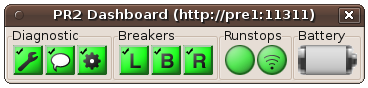
\includegraphics[scale=0.5]{dashboard3.png}
\caption{The PR2 dashboard when the wireless run-stop is in the start position.}
\label{fig:dashboard3}
\end{figure}

If this calibration step fails, then you can use the pr2\_dashboard to diagnose the problems with the robot. See your robot administrator if you need assistance in understanding and addressesing the issues.

\section{Tucking the robot arms}

Before driving a robot around, it is best to tuck the robot arms. If you do not tuck the robot arms before driving, then the arms are likely to swing around while the robot is moving.

To run the tuckarm package, type into the robot computer (pr\textless x\textgreater 1):
\begin{verbatim}
$ rosrun pr2_tuckarm tuckarm.py b
\end{verbatim}
This will tuck both robot arms. The feedback from tuckarm should display something like this:
\begin{verbatim}
[INFO] 1264099125.710039: Waiting for controller manager to start
[INFO] 1264099125.718283: Tucking both left and right arm
\end{verbatim}

For more information about how to drive the robot around, see the 
\href{http://www.ros.org/wiki/pr2_tuckarm}{tuckarm} instructions at \href{http://www.ros.org}{ros.org}.

\section{Driving with the joystick}
To move the robot, you can now drive it around with the joystick.  To do this, you will need to open a new terminal window with a new ssh connection 
to the robot and run the teleop\_joystick launch file
\begin{verbatim}
$ ssh <username>@pr<x>1
$ roslaunch pr2_teleop teleop_joystick.launch 
\end{verbatim}

Be sure to check to see if the robot is plugged in (e.g., ethernet cables or power cables)! If it is plugged in, then be very cautious to avoid pulling the cables out improperly.

Once the teleop\_joystick node is running, press the pairing button (Figure~\ref{fig:ps3_pairing}) in the middle of the 
joystick to pair it with the robot. Be sure to unplug the robot from wall outlets if you are going to drive the robot around. 
\begin{figure}[H]
\centering
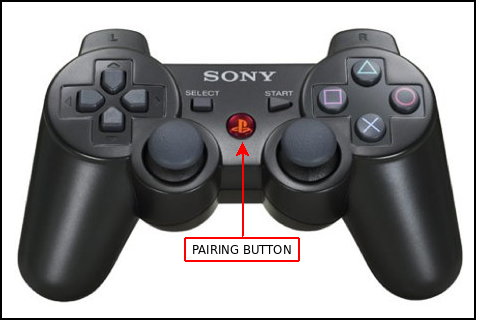
\includegraphics[scale=0.40]{pairing.png}
\caption{Pairing the joystick with the PR2.}
\label{fig:ps3_pairing}
\end{figure}
Then to control the robot, use L1 (Figure~\ref{fig:buttons}) as the ``deadman'' switch. L1 should be held down with your left pointer finger (like a trigger) whenever you wish to control the robot. If you let go of the L1 button, then commands will no longer be sent from the controller to the robot. While pressing L1, use the other buttons for the following movements:
\begin{figure}[H]
\centering
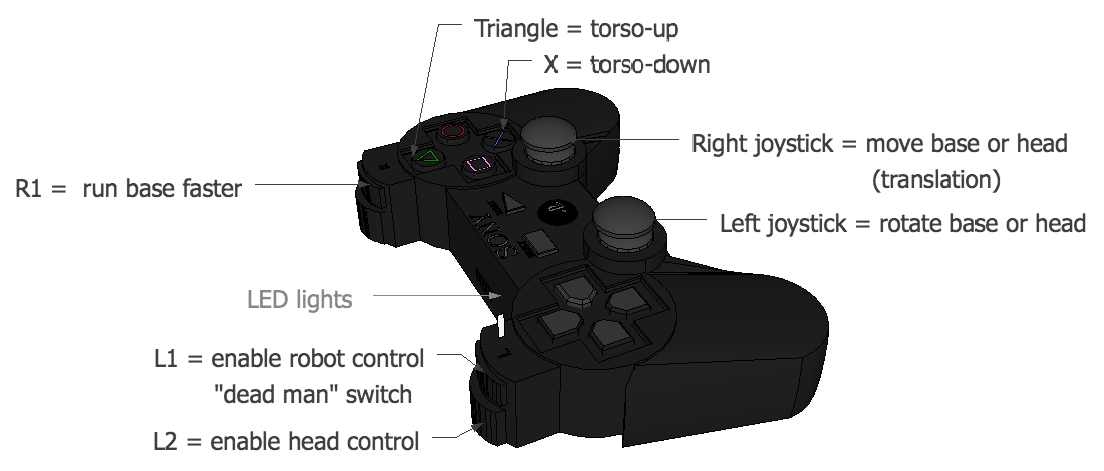
\includegraphics[scale=0.3]{ps3diagram.png}
\caption{The PS3 controller mapped to robot movements.}
\label{fig:buttons}
\end{figure}
\begin{enumerate}
\item L1 (left pointer finger): The ``dead man'' switch allows the controller to send commands to the robot
\item L2 (right pointer finger): The head switch allows the joysticks to control the head instead of the base
\item Right joystick (right thumb): Translates the base or head (i.e., front, back, left, right)
\item Left joystick (left thumb): Rotates the base or head (i.e., spin clockwise or counter-clockwise)
\item R1 (left pointer finger): The ``run'' switch commands the base to move faster
\item Triangle and X (right thumb): Moves the torso up and down 
\end{enumerate}

To drive the robot around (i.e., driving the base), hold down L1 and use the two joysticks to control its direction of movement (right joystick) and rotation (left joystick). To drive the robot around at faster speeds, also hold down R1.

To move the robot head, hold down L1 and use the two joysticks to control the head movements.

To move the robot torso, hold down L1 and press the triangle button to move the torso up or the X button to move the torso down. The torso moves slowy.

For more information about how to drive the robot around, see the 
\href{http://www.ros.org/wiki/ps3joy/Tutorials/UsingJoystickWithPR2}{ps3joy} tutorial at \href{http://www.ros.org}{ros.org}. 

\section{Visualizing sensor data}
To see the sensor data from the robot, you can use rviz on the offboard computer (e.g., base station).  Again, you will 
need to open a new terminal window and configure the ROS\_MASTER\_URI to point at the robot, so run
\begin{verbatim}
$ export ROS_MASTER_URI=http://pr<x>1:11311
$ rosrun rviz rviz
\end{verbatim}
and you should see rviz launch with a visualization of the robot.\footnote{If you do not see rviz appear, then there is a chance that you have not yet built rviz yet. To do this, type \texttt{rosmake rviz} to build rviz. Once this is done, you can try launching rviz again.}

For more information about how to view different types 
of data coming from the robot, see the \href{http://ros.org/wiki/rviz}{rviz} documentation at 
\href{http://www.ros.org}{ros.org}.
(TODO - WITH THE CURRENT LAUNCH FILE, YOU WILL NOT BE ABLE TO SEE CAMERA DATA)

\section{What next?}
From here, you can do what you want on the robot.  (NOTE TO AUTHORS: Point to instructions for writing code and to a list of other 
applications and things to do with the robot.)

\section{Putting Away the PR2}
To properly put away the PR2, you should drive the robot to the appropriate location in your lab, plug in the robot to recharge the batteries,
press STOP on the wireless run-stop, stop the processes on the robot, and log off of the robot.

First, put away the robot. Drive the robot to the appropriate location in your lab and plug it in to recharge.
% Add notes here about how to recharge the robot without getting shocked.

Second, stop all the processes running on the robot. If you want to stop all of the processes running on the robot and log off of the robot, but not turn off the robot computers, then open a new terminal and type:
\begin{verbatim}
$ ssh <username>@pr<x>1
$ sudo robot stop
\end{verbatim}
This logs you into the robot and stops the robot processes.

As an alternative to simply stopping the proceeses running on the robot, you can also turn off the robot computers. To do this, open a new terminal and type:
\begin{verbatim}
$ ssh <username>@pr<x>1
$ sudo pr2-shutdown
\end{verbatim}

If you turn off the robot, you will hear four sets of descending beeps from the robot computers. Then the red lights on each of the computers will turn off. If this does not happen, then the robot computers might not be completely shut down properly.

Finally, to exit from the robot computer terminal, type
\begin{verbatim}
$ exit
\end{verbatim}

If someone was waiting to use the robot after you, be sure to let them know that you are done with the robot.
